\documentclass[a4paper,12pt]{article} 

%%% Работа с русским языком
\usepackage{cmap}                           % поиск в PDF
\usepackage{mathtext} 			 	       % русские буквы в формулах
\usepackage[T2A]{fontenc}               % кодировка
\usepackage[utf8]{inputenc}              % кодировка исходного текста
\usepackage[english,russian]{babel}  % локализация и переносы
\usepackage{wrapfig}
\usepackage{gensymb}
\usepackage{textcomp}
\usepackage{multirow}
\usepackage{amsmath,amsfonts,amssymb,amsthm,mathtools} % AMS
\usepackage{euscript}	 % Шрифт Евклид
\usepackage{mathrsfs} % Красивый матшрифт
\usepackage{graphicx}%Вставка картинок правильная
\usepackage{float}%"Плавающие" картинки
\usepackage{wrapfig}%Обтекание фигур (таблиц, картинок и прочего)
\title{Лабораторная работа 2.4.1 

Определение теплоты испарения жидкости}
\author{Кагарманов Радмир Б01-106}
\date{18 мая 2022 г.}

\begin{document}

\maketitle
\thispagestyle{empty}
\newpage
\setcounter{page}{1}
\paragraph{Цель работы:}: 1) измерение давления насыщенного пара жидкости
при разной температуре; 2) вычисление по полученным данным теплоты испарения с помощью уравнения Клапейрона–Клаузиуса.
\paragraph{В работе используется:}термостат; герметический сосуд, заполненный исследуемой жидкостью; отсчётный микроскоп.
\paragraph{Теоретические сведения\\}
Теплоту парообразования жидкостей можно измерить непосредственно при помощи калориметра. Такой метод, однако, не позволяет
получить точных результатов из-за неконтролируемых потерь тепла,
которые трудно сделать малыми. В настоящей работе для определения
теплоты испарения применен косвенный метод, основанный на формуле
Клапейрона–Клаузиуса:
\begin{equation}
    \frac{dP}{dT}=\frac{L}{T(V_2-V_1)}
\end{equation}
Здесь $P$ - давление насыщенного пара жидкости при температуре $T$, $T$ - абсолютная температура жидкости и пара, $L$ - теплота испарения жидкости, $V_2$ - объём пара, $V_1$ - объём жидкости. Найдя из опыта $\frac{dP}{dT}, ~V_2, ~V_1~ и ~T$, можно определить $L$ путём расчёта. Величины $L, ~V_2, ~V_1$ в формуле (1) должны относиться к одному и тому же количеству
вещества; мы будем относить их к одному молю. \\
При давлениях ниже атмосферного уравнение Ван-дер-Ваальса для насыщенного пара мало отличается от уравнения Клапейрона. Положим
поэтому:
\begin{equation}
    V=\frac{RT}{P}
\end{equation}
Подставляя (2) в (1), пренебрегая $V_1$ и разрешая уравнение относительно L, найдём:
\begin{equation}
    L=\frac{RT^2}{P}\frac{dP}{dT}=-R\frac{d(ln ~P)}{d(1/T)}
\end{equation}
\paragraph{Экспериментальная установка\\}
Схема
установки изображена на рис. 1. Наполненный водой резервуар 1 играет роль термостата. Нагревание термостата производится
спиралью 2, подогреваемой электрическим
током. Для охлаждения воды в термостате через змеевик 3 пропускается водопроводная вода. Вода в термостате перемешивается воздухом, поступающим через трубку 4. Температура воды измеряется термометром 5. В термостат погружён запаянный прибор 6 с исследуемой
жидкостью. Над ней находится насыщенный пар (перед заполнением
прибора воздух из него был откачан). Давление насыщенного пара определяется по ртутному манометру, соединённому с исследуемым объёмом. Отсчёт показаний манометра производится при помощи микроскопа.
\begin{figure}[!h]
\centering
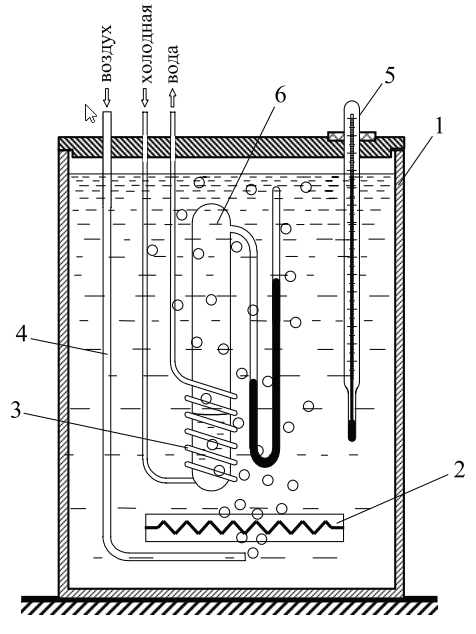
\includegraphics[width=0.55\linewidth]{Уст.png}
\caption{Экспериментальная установка}
\label{fig:mpr}
\end{figure}
\paragraph{Обработка результатов\\}
\subparagraph{1.} Построим графики зависимости $ln~P$ от $1/T$. Они изображёны на Рис. 2. В таблицах 1 и 2 приведены значения разницы высоты столбцов ртутного манометра и температуры. 
\begin{figure}[!h]
\centering
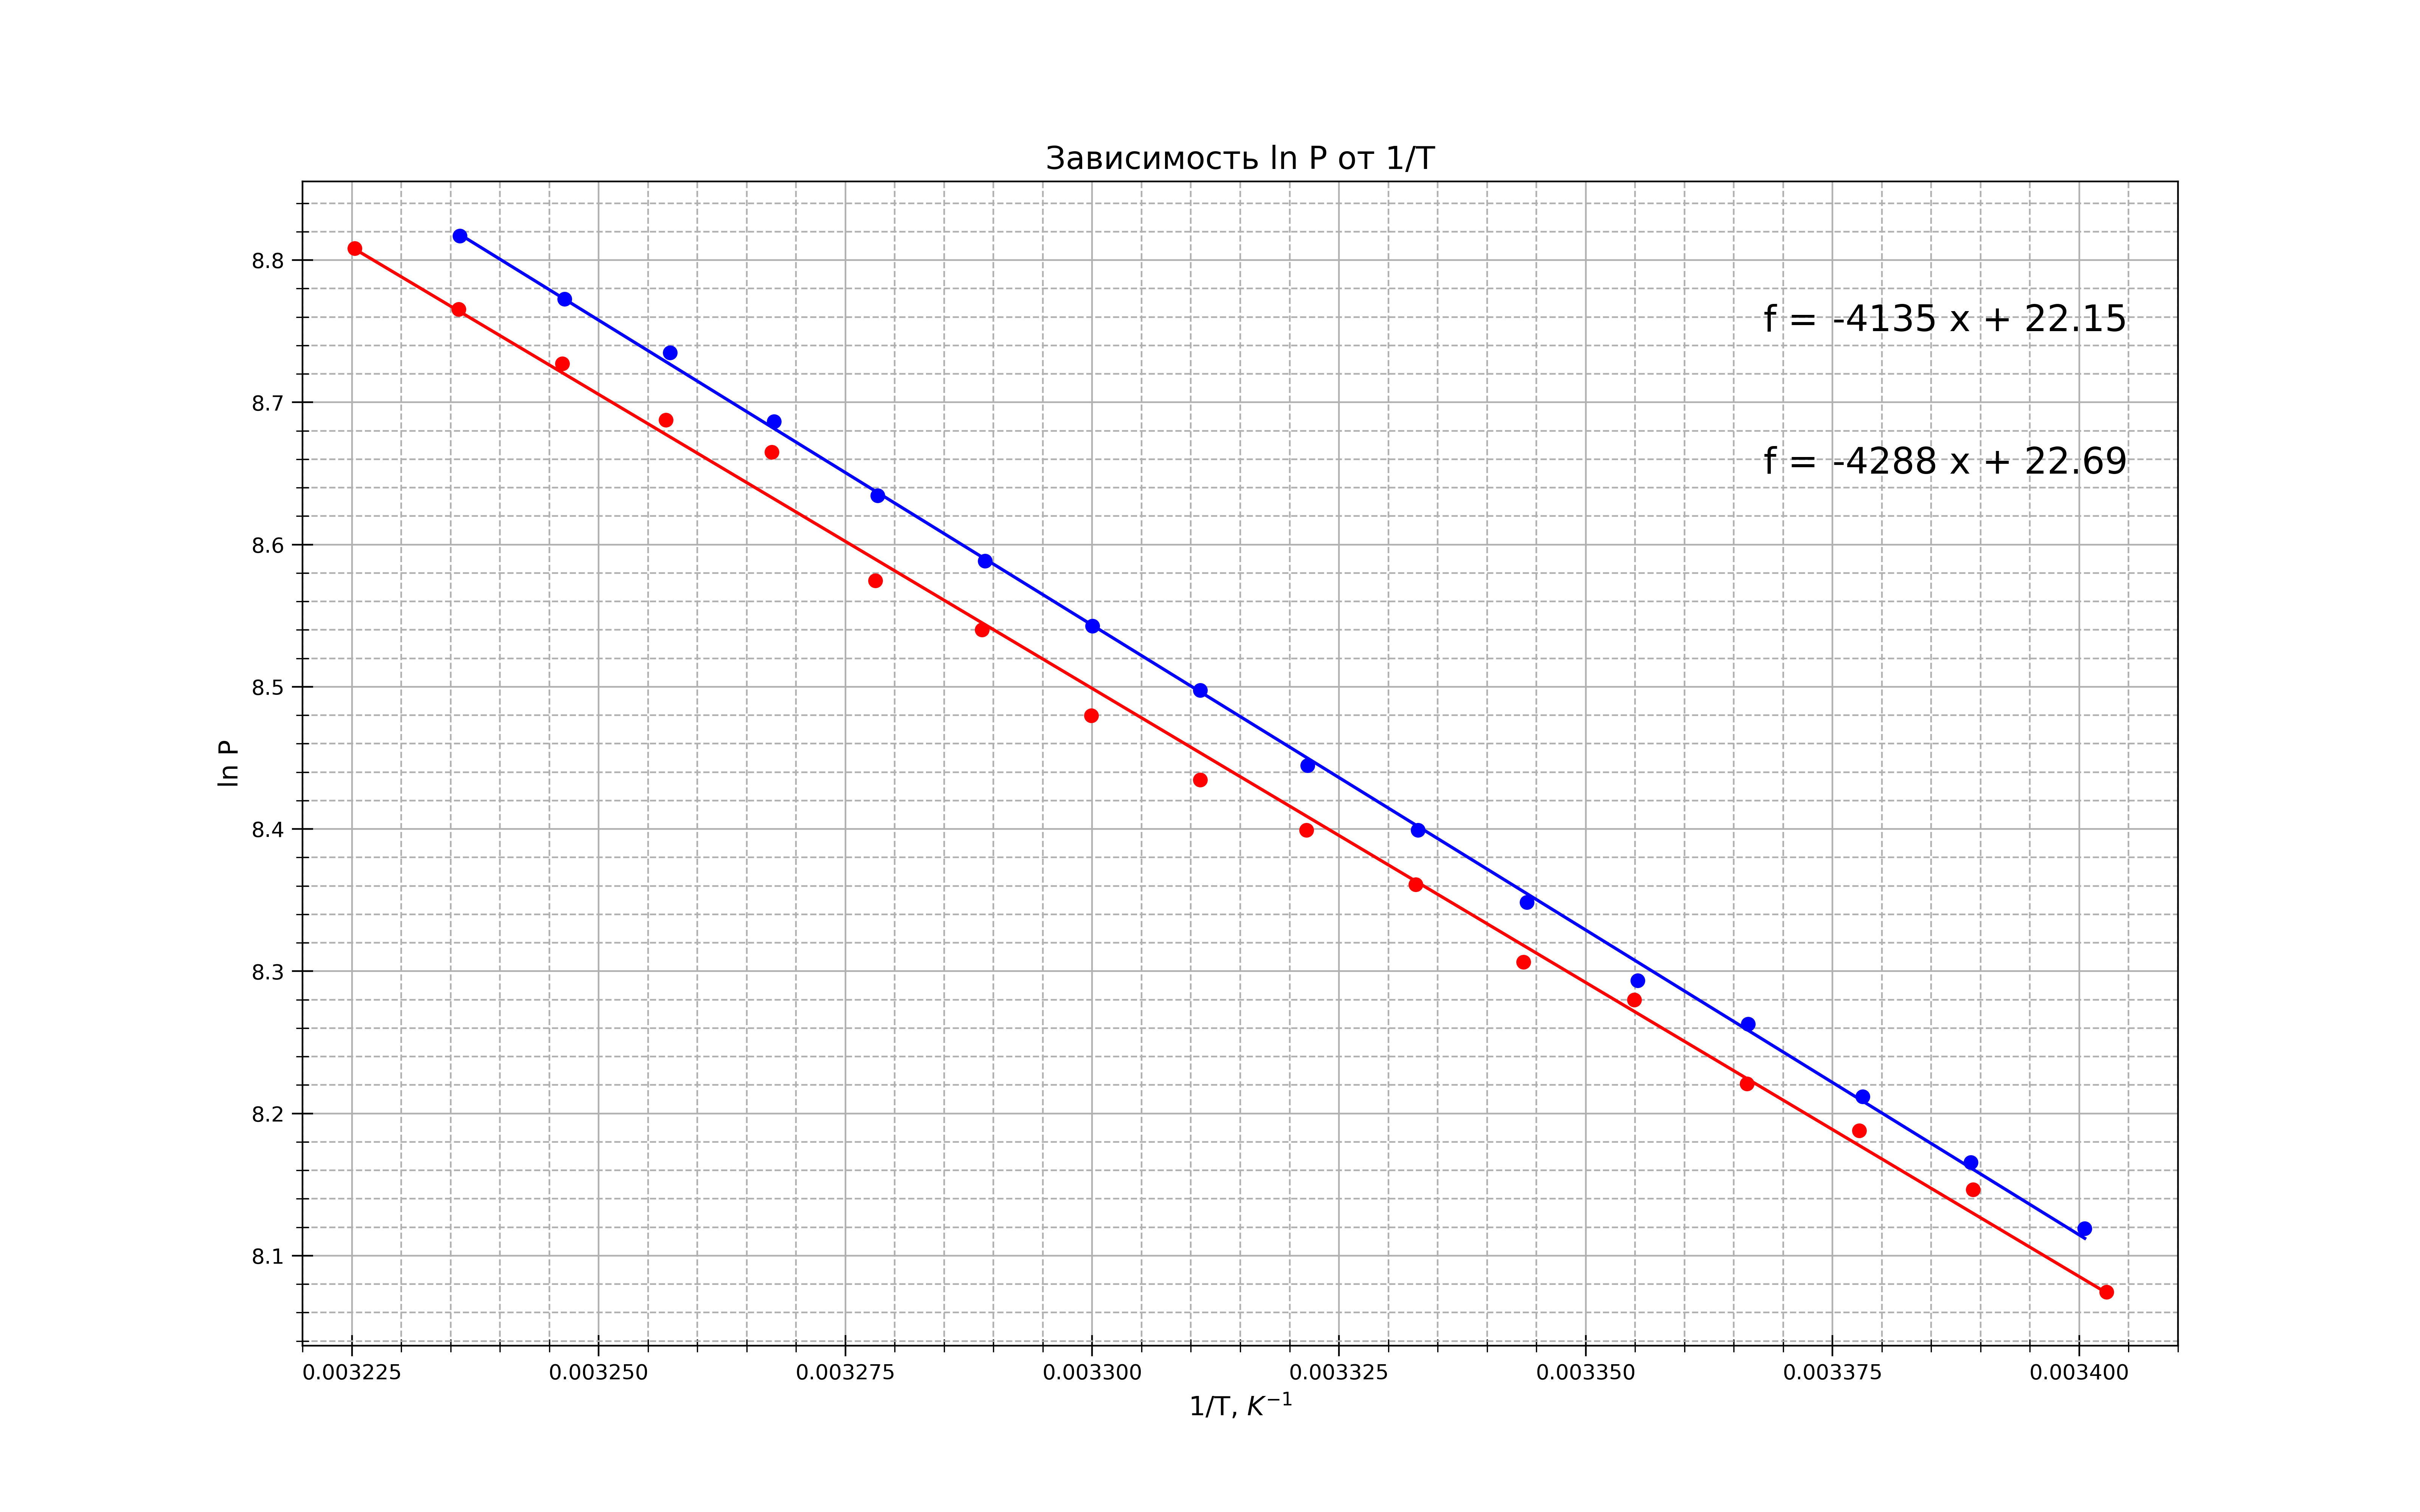
\includegraphics[width=0.9\linewidth]{graph.png}
\caption{Экспериментальная установка}
\label{fig:mpr}
\end{figure}
\newpage
С помощью метода наименьших квадратов найдём $\frac{d(ln~P)}{d(1/T)}$:
\begin{center}
    При нагревании: $k_{н} = -4135\pm 138~ K$\\
    При охлаждении: $k_{о} = -4288\pm 132~ K$
\end{center}\\
\subparagraph{2.} По формуле (3) посчитаем $L$:
\begin{center}
    $L_{н}=34,4\pm 1,1~\frac{кДж}{моль}$\\
    $L_{о}=35,6\pm 1,1~ \frac{кДж}{моль}$
\end{center}
Для сравнения с табличным значением $L$ перейдём к удельной теплоте:
\begin{center}
    $L_{н}=1,91\pm 0,06~\frac{МДж}{кг}$\\
    $L_{о}=1,98\pm 0,06~ \frac{МДж}{кг}$\\
    $L_{табл}=2,26~ \frac{МДж}{кг}$
\end{center}
\paragraph{Вывод:}в данной работе мы вычислили теплоту парообразования воды с помощью увеличения и понижения температуры. Более точный результат получился при понижении $L_{о}=1,98\pm 0,06~ \frac{МДж}{кг}$. Табличное значение $L=2,26~ \frac{МДж}{кг}$.\\
\begin{table}[h]
    \centering
    \begin{tabular}{|c|c|} \hline
    $T, K$ & $\Delta h, см$ \\ \hline
         293,88 & 2,41 \\ \hline
         295,05 & 2,59 \\ \hline
         296,06 & 2,7 \\ \hline
         297,06 & 2,79 \\ \hline
         298,07 & 2,96 \\ \hline
         299,07 & 3,04 \\ \hline
         300,05 & 3,21 \\ \hline
         301,05 & 3,335 \\ \hline
         302,03 & 3,455 \\ \hline
         303,04 & 3,615 \\ \hline
         304,06 & 3,84 \\ \hline
         305,06 & 3,975 \\ \hline
         306,04 & 4,35 \\ \hline
         307,05 & 4,45 \\ \hline
         308,04 & 4,63 \\ \hline
         309,04 & 4,81 \\ \hline
         310,05 & 5,02 \\ \hline
    \end{tabular}
    \caption{Нагрев}
    \label{tab:my_label}
\end{table}
\begin{table}[h]
    \centering
    \begin{tabular}{|c|c|} \hline
    $T, K$ & $\Delta h, см$ \\ \hline
         309,03 & 5,065 \\ \hline
         308,02 & 4,845\\ \hline
         307,01 & 4,665\\ \hline
         306,02 & 4,445\\ \hline
         305,04 & 4,22\\ \hline
         304,03 & 4,03\\ \hline
         303,03 & 3,85\\ \hline
         302,03 & 3,68\\ \hline
         301,04 & 3,49\\ \hline
         300,03 & 3,335\\ \hline
         299,04 & 3,17\\ \hline
         298,04 & 3\\ \hline
         297,05 & 2,91\\ \hline
         296,03 & 2,765\\ \hline
         295,07 & 2,64\\ \hline
         294,07 & 2,52\\ \hline
    \end{tabular}
    \caption{Охлаждение}
    \label{tab:my_label}
\end{table}
\end{document}
